\documentclass[a4paper]{article}


\usepackage{alphabeta} 
\usepackage{enumitem} 
\usepackage{mathtools}
\usepackage{amsmath, amssymb} 
\usepackage{amsthm}
\usepackage{cancel} 
\usepackage[margin=0.70in]{geometry} 
\geometry{left=3cm,right=3cm,top=2.4cm,bottom=2.4cm}	%the page geometry as defined, A4=210x297mm
\usepackage{graphicx}
\usepackage{wrapfig}
\usepackage{caption}
\usepackage{textcomp}
\usepackage{tabto}
\usepackage{layout}
\usepackage{bm}
\usepackage{minipage-marginpar}
\usepackage[dvipsnames]{xcolor}
\usepackage{hyperref}
\usepackage{dutchcal}
\usepackage{derivative}
\usepackage{esint}
%\usepackage{biblatex}
\usepackage{subcaption}
\usepackage{booktabs}\usepackage{derivative}
\usepackage[flushleft]{threeparttable}
\usepackage[capbesideposition=outside,capbesidesep=quad]{floatrow}
\usepackage{derivative}
\usepackage[thinc]{esdiff}
\usepackage{lipsum}
\usepackage{arydshln}
%%RENEW

\newtheorem{problem}{Άσκηση}
\newtheorem*{solution*}{Λύση}
\newtheorem{definition}{Ορισμός}[subsection]
\newtheorem{properties}{Ιδιότητες}[subsection]
\newtheorem{theorem}{Θεώρημα}[subsection]
\newtheorem{protash}{Πρόταση}[subsection]
\newtheorem{porisma}{Πόρισμα}[subsection]
\newtheorem{lemma}{Λήμμα}[subsection]
\newtheorem*{prooof}{Απόδειξη}
\newtheorem*{notes}{Παρατηρήσεις}
\newtheorem*{note}{Παρατήρηση}
\newtheorem*{app}{Εφαρμογή} 
\newtheorem*{example}{Παράδειγμα}
\newtheorem*{examples}{Παραδείγματα}


\newcommand\numberthis{\addtocounter{equation}{1}\tag{\theequation}}
%\renewcommand{\labelenumi}{\roman{enumi}}
\newcommand{\approxtext}[1]{\ensuremath{\stackrel{\text{#1}}{\approx}}}
\renewcommand{\figurename}{Εικόνα.}
\renewcommand{\tablename}{Πίνακας.}
%\renewcommand\refname{New References Header}
\renewcommand*\contentsname{Περιεχόμενα}
%\DeclareDerivative{\odv}{\mathrm{d}}


\begin{document}
\begin{titlepage}			%makes a title page. Remember to change the author, CID, username and group number to what is appropriate for you!
	\centering
	{\scshape\LARGE Εθνικό Μετσόβιο Πολυτεχνείο\par}
	{\scshape \LARGE Σ.Ε.Μ.Φ.Ε.\par}
	\vspace{1cm}
	{\huge\bfseries Περίθλαση Ακτίνων X \par}
	\vspace{1cm}
	{\Large\itshape Θωμόπουλος Σπύρος\par}		%remember to change these!
	
	%		{\large Group \@group\unskip\strut\par}
	{\large spyros.thomop@gmail.com/ ge19042@mail.ntua.gr\par \hfill \\}% 		%remember to change these!
	\vspace{1cm}
	{\large Ημερμονηνία Παράδοσης 03/05/2022\par}
\end{titlepage}


\subsection*{Σκοπός}	
	Ο σκοπός της εν λόγω εργαστηριακής άσκησης είναι η μελέτη του φαινομένου της περίθλασης των ακτινών Χ από μονοκρυστάλλους, μέσω της οποίας μπορούμε να υπολογίσουμε την σταθερά του Planck, αλλά και την απόσταση μεταξύ των πλεγματικών επιπέδων ενός κρυστάλλικού στερεού.
	
\subsection*{Θεωρητικά Στοιχεία}
	\subsubsection*{Παραγωγή Ακτίνων Χ}
	
		Οι ακτίνες Χ παράγονται στον λεγόμενο σωλήνα Coolidge. Μέσα σε αυτόν επικρατούν συνθήκες υψηλού κενού $(\sim10^{-7}atm)$ και υπάρχει μία κάθοδος (χαμηλού δυναμικού) από την οποία εκπέμπονται ηλεκτρόνια μέσω της θερμιονικής εκπομπής και μία άνοδος (υψηλού δυναμικού) από Χαλκό. Έχουμε δύο τρόπους με τους οποίους παίρνουμε ακτίνες Χ. Αρχικά, υπάρχουν τα ηλεκτρόνια που επιβραδύνονται από την άνοδο και η ενέργειά τους μετατρέπεται αμέσως σε φωτόνια με συνεχές φάσμα, στα οποία περιλαμβάνονται και φωτόνια ακτινών Χ (ακτινοβολία πέδησης). Εδώ υπάρχει ένα ελάχιστο μήκος κύματος εκπομπής $(\lambda_{min})$ το οποίο προέρχεται από ηλεκτρόνια που έχουν χάσει όλη τους την κινητική ενέργεια κατά την σύγκρουση με την άνοδο και το οποίο γίνεται μεγαλύτερο όσο μεγαλώνουμε την διαφορά δυναμικού ανόδου-καθόδου, αυτό διότι έχουμε 
		\begin{align*}\label{1}
			E = h f = h \frac{c}{\lambda} \xRightarrow{E_{max}=eV} \lambda_{min} = \frac{hc}{eV} \numberthis
		\end{align*}
		
	Κάποια άλλα ηλεκτρόνια μεταφέρουν ποσό της ενέργειάς τους σε συγκεκριμένα άτομα της ανόδου διεγείροντάς σε ανώτερες ενεργειακές καταστάσεις. Καθώς αυτά τα άτομα αποδιεγείρονται, μέσω αυθόρμητης αποδιέγερσης, στις βασικές τους ενεργειακές καταστάσεις, θα έχουμε εκπομπή φωτονίων. Συγκεκριμένα, αν τα διεγειρόμενα ηλεκτρόνια ανήκουν σε εσωτερικές στοιβάδες τότε τα εκπεμπόμενα φωτόνια ανήκουν στην κατηγορία των ακτίων Χ. Τότε έχουμε και το \textit{χαρακτηριστικό φάσμα εκπομπής ακτίνων Χ} του υλικού της ανόδου. 
	
	Πιο ειδικά, αν έχουμε τις μεταβάσεις $2p\rightarrow1s$ και $3p\rightarrow1s$ παίρνουμε ενέργειες $K_\alpha$, $K_\beta$ αντίστοιχα, οι οποίες ισούνται με την διαφορά των ενεργειών των σταθμών μεταξύ των οποίων γίνεται η μετάβαση.
	
	\subsubsection*{Περίθλαση Bragg}
	
	Αφού πετύχουμε την παραγωγή των ακτίνων Χ, θέλουμε να τις χρησιμοποιήσουμε προκειμένου να ανιχνεύσουμε την εσωτερική κρυσταλλική δομή ενός στερεού και να μετρήσουμε την απόσταση των κρυσταλλικών επιπέδων μέσω της ανάκλασης Bragg.
	
	O Bragg, θεώρησε τα κρυσταλλικά επίπεδο ως ημιπερατά οπτικά κάτοπτρα στα οποία προσπίπτει η ακτινοβολία Χ υπό γωνία $\theta$, η οποία διέρχεται και ανακλάται. Οι ανακλώμενες ακτίνες από τα γειτονικά επίπεδα συμβάλλουν και για να έχουμε ενίσχυση πρέπει να ισχύει η συνθήκη Bragg
\begin{align*}\label{2}
2dsin\theta=m\lambda \numberthis
\end{align*}
όπου $\lambda$ το μήκος κύματος της εισερχόμενης δέσμης, d η απόσταση των διαδοχικών επιπέδων και $m\in \mathbb{N}$ η τάξη της περίθλασης. 
%Η ίδια ανάλυση γίνεται αν αντικαταστήσουμε τις ακτίνες Χ με ηλεκτρόνια. Επίσης η μέθοδος δουλεύει για μονοχρωματικές ακτίνες Χ και κατ' αντιστοιχία με δέσμη ηλεκτρονίων που έχει μικρή διασπορά $\sim 0.01\%$ στην ταχύτητα.
\begin{figure}[h!]-
	\centering
	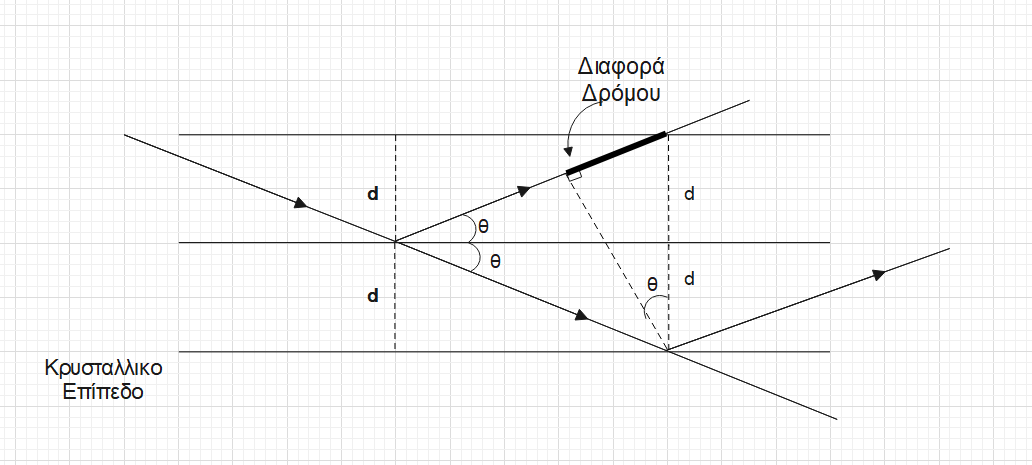
\includegraphics[scale=0.4]{bragg.png}
\end{figure}

Κατ' αυτόν τον τρόπο, γνωρίζοντας το μήκος κύματος $\lambda$, την τάξη m της περίθλασης και μετρώντας πειραματικά την γωνία $\theta$ μπορούμε να υπολογίσουμε την απόσταση μεταξύ των πλεγματικών επιπέδων του κρυστάλλου

	
\subsection*{Πειραματική Διάταξη}
Η πειραματική διάταξη αποτελείται από 
\begin{itemize}
	\item[.] Σωλήνα Coolidge για παραγωγή ακτίνων Χ από χαλκό
	\item[.] Έναν κρύσταλλο (LiF) και το σύστημα περιστροφής του
	\item[.] Ανιχνευτή Geiger-Muller με γωνιόμετρο
	\item[.] Μόνάδα λήψης δεδομένων \& Η/Υ
\end{itemize}

\begin{figure}[h!]
	\centering
	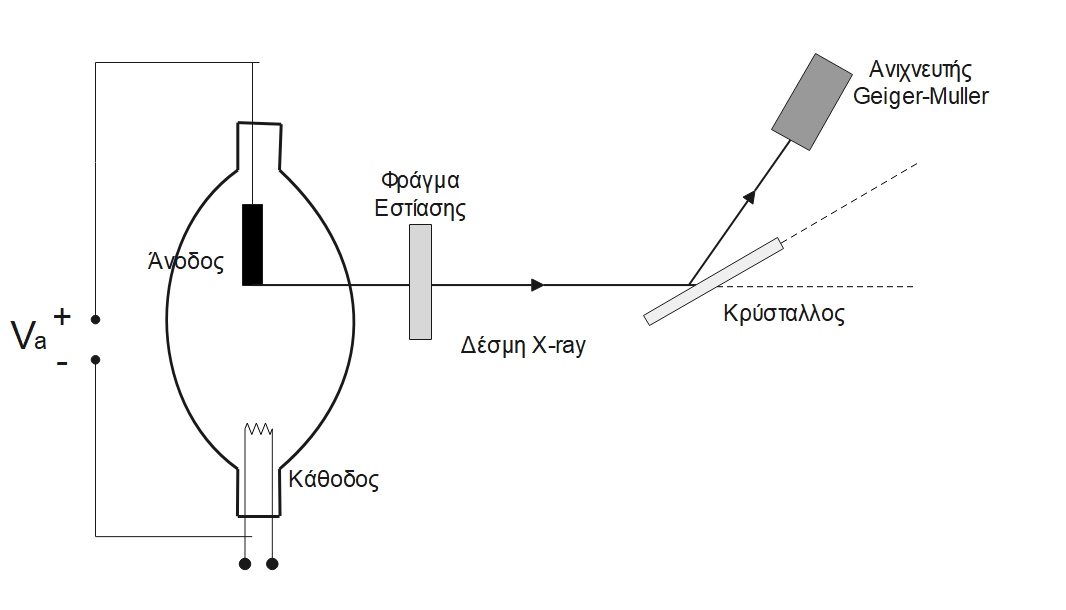
\includegraphics[scale=0.3]{setup.png}
	\caption{ Η πειραματική διάταξη}
\end{figure}
\subsection*{Πειραματική Διαδικασία - Επεξεργασία Μετρήσεων}

\subsubsection*{Μέρος Α: Υπολογισμός της σταθεράς του Planck}
	Αφού ενεργοποιήσουμε όλες τις συσκευές της διάταξης και τοποθετήσουμε στην συσκευή τον κρύσταλλο LiF, ανοίγουμε το αντίστοιχο πρόγραμμα στον ΗΥ. Τώρα επιλέγουμε τιμή διαφοράς δυναμικού ανόδου-κοθόδου $34kV$, γωνία περιστροφής $4-65^o$ και βήμα αύξησης $\Delta\theta=0.1^o$. Καταγράφουμε το μήκος κύματος $\lambda_{min}$ και έπειτα επαλαμβάνουμε τις μετρήσεις για τάσεις $32-18kV$ με βήμα $2kV$. Τα αποτελέσματα φαίνονται στον Πίνακα 1. 
	\begin{table}[h!]
		\centering
		\begin{tabular}{r|r|r|r}
		$V(\pm0.1kV)$ & $1/V(10^{-5}V^{-1})$ & $\lambda_{min}(pm)$ & $\Delta\lambda (pm)$ \\ 
		\hline\hline
		34&2.94&35.81&0.01\\
		32&3.13&37.21&0.01\\
		30&3.33&39.31&0.01\\
		28&3.57&43.50&0.01\\
		26&3.85&44.90&0.01\\
		24&4.17&47.69&0.01\\
		22&4.55&52.57&0.01\\
		20&5.00&58.84&0.01\\
		18&5.56&63.01&0.01
		\end{tabular}
	\end{table}
	
	Εφρομόζοντας την μέθοδο των ελαχίστων τετραγώνων για $X=1/V$ και $Y = \lambda_{min}$, προκύπτει μία ευθεία που την εξαναγκάζουμε να περνάει από την αρχή των αξόνων λόγω της σχέσης (\ref{1}), $Y=A\cdot X$, με: 
	\begin{align}
		A = ( 11.67 \pm 0.10) [pm\cdot10^5V]
	\end{align}
	
	Οι συντελεστές και τα σφάλματά τους πρκύπτουν από τις σχέσεις 
	\begin{align*}
		A &= \frac{\sum_{i=1}^{n}x_iy_i}{\sum_{i=1}^{n}x_i^2}
		%B &= \frac{N\sum_{i=1}^{N}x_iy_i-\sum_{i=1}^{N}x_i\sum_{i=1}^{N}y_i}{D} \\ 
		%D &= N\sum_{i=1}^{N}x_i^2-\left( \sum_{i=1}^{N}\right)^2
	\end{align*}
	και 
	\begin{align*}
		(\delta A)^2=\sigma_A^2=\frac{\sigma_y^2}{\sum_{i=1}^{n}x_i^2}, \hspace{1.0cm}\text{με} \hspace{0.3cm} 
        \sigma_y\simeq\sum_{i=1}^{n}\frac{(y_i-bx_i)^2}{n-1}
	\end{align*}
		%\delta A &= \sigma_y \sqrt{\frac{\sum_{i=1}^{N}x_i^2}{D}} \\ 
		%\delta B &= \sigma_y \sqrt{\frac{N}{D}} \\ 
		%\sigma_y &= \sqrt{\frac{\sigma_{i=1}^{N}(y_i-A-Bx_i)^2}{N-2}}
	Προκύπτει η γραφική παράσταση που φαίνεται στην Εικόνα 2.
	\begin{figure}[h!]
		\centering
		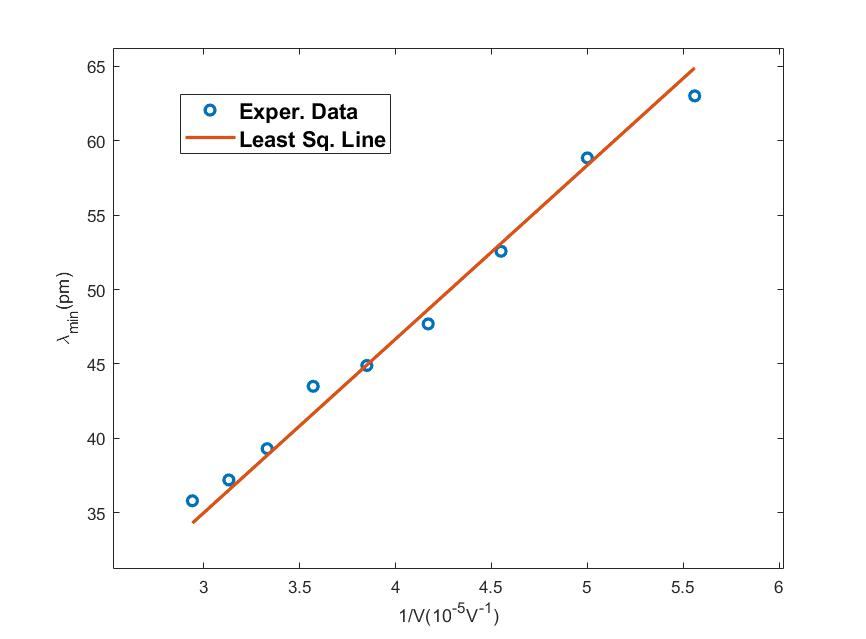
\includegraphics[scale=0.4]{plot1.jpg}
		\caption{ $1/V - \lambda_{min}$}
	\end{figure}
	Αν λύσουμε την σχέση (\ref{1}) ως προς $\lambda_{min}$ προκύπτει μία ευθεία με κλίση η οποία ισούται με αυτή που προέκυψε από την μέθοδο ελαχίστων τετραγώνων και από την οποία μπορούμε να υπολογίσουμε την σταθερά του Planck:
		\begin{align*}
			A = \frac{hc}{e} \Rightarrow h = \frac{eA}{c} = 6.24 \times 10^{-34} Js
		\end{align*}
		με σφάλμα από διάδοση 
	\begin{align*}
		\delta h = \sqrt{\left( \pdv{h}{A}\delta A\right)^2} = \frac{e\delta A}{c} = 0.05 \times10^{-34}Js
	\end{align*}
	Άρα έχουμε $h = (6.24\pm0.05)\times10^{-34}J s$.
	Παρατηρώ ότι συμπιπτει στα όρια του σφάλματος με την αποδεκτή τιμή της σταθεράς που είναι $h=6.62\times10^{-34}Js$. Σφάλματα που οδηγούν στην απόκλιση ίσως είναι κυρίως η πολυκαιρία του κρυστάλλου liF.
	
	\subsubsection*{Μέρος Β: Απόσταση Πλεγματικών Επιπέδων}
	Τοποθετούμε στην συσκευή τον κρύσταλλο KBr, εφαρμόζουμε τάση ανόδου-καθόδου $V=18kV$ και καταγράφουμε το φάσμα συναρτήσει της γωνίας που βρίσκεται ο ανιχνευτής G-M. Εκεί παρατηρούμε διάφορα μέγιστα τα οποία φαίνονται στον Πίνακα 2.
	\begin{table}[h!]
		\centering
		\begin{tabular}{r|c|r|r|r}
			$\theta(\pm0.2^o)$ & Τύπος Ακτιν. & $\lambda_{theor}(pm)$ & Τάξη Περίθλ. & $d(pm)$ \\ 
			\hline\hline
			12.8 & $K_{\alpha}$  & 154.3 & 1 & 348.2\\
			14.2 & $K_{\beta}$ & 139.3 & 1 & 284.0\\	
			25.6 & $K_{\alpha}$  & 154.3 & 2 & 357.1\\
			28.8 & $K_{\beta}$ & 139.3 & 2 & 289.2		
		\end{tabular}
	\end{table}
	
		Η απόσταση d των πλεγματικών επιπέδων υπολογίζεται από την σχέση του Bragg (\ref{2}). Κατά μέσο όρο έχουμε 
		\begin{align*}
			d_{Cu} = (319.6 \pm 38.4) [pm]
		\end{align*}
		Η αναμενόμενη τιμή είναι $d_{Cu,expexcted}=329.0pm$. Συνεπως, αυτή που βρέθηκε πειραματικά συμπίπτει στα όρια του σφάλματός της με την αναμενόμενη. Δεδομένου στην εν λόγω άσκηση δεν έχουμε κάνει κάποιον χειροκίνητο χειρισμό της διάταξης αλλά μόνο μέσω του Η/Υ, το πιό πιθανό αίτιο για την απόκλιση που παρατηρουμε είναι η φθορά του κρυστάλλου KBr από την πολυκαιρία.

\end{document}